\section{Descriptors}
\frame{
    \begin{block}{}
        \centering
        Topological Descriptors
    \end{block}
}

\frame{
    \frametitle{Stat Reverences}

    \begin{block}{}
        Wasserman. All of Statistics: a Concise Course in Statistical Inference.
        Springer, 2010.\\~\\
        Givens and Hoeting. Computational Statistics. Wiley, 2013.
    \end{block}
}

\frame{
    \frametitle{Stat Slide: The Basics}

    \begin{block}{}
        \begin{itemize}
            \onslide<1->{\item Let $F$ be a probability distribution with
                density $f$.}%
            \onslide<2->{\item $X \sim F$ reads ``$X$ has distribution $F$".}%
            \onslide<2->{\item Here, $X$ is called a \emph{random variable}.}
            \onslide<3->{\item Expectation: $\mathbb{E}(X) = \int x \,dF(x)$.}
            \onslide<4->{\item Quantile Function $\textsc{CDF}^{-1}(q)$.}
        \end{itemize}

            \centering
            \only<1-3>{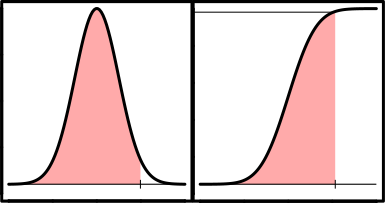
\includegraphics[width=3in]{figs/stat/pdfcdf}}%
            \only<4>{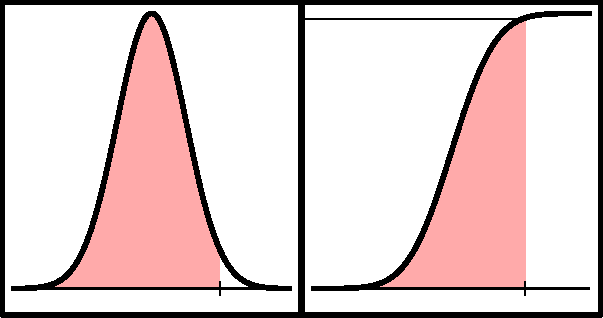
\includegraphics[width=3in]{figs/stat/pdfcdf-quantile}}%
    \end{block}
}

\frame{
    \frametitle{Prob/Stat Slide: Descriptors and Limit Theory}

    \begin{block}{}
        \begin{itemize}
            \item Let $F$ be some distribution.
            \item Let $X_1, X_2, \ldots, X_n \sim F$. (The data). \pause
            \item A \emph{statistic} or \emph{descriptor} is a function of the data:\\
                $T(X_1, X_2, \ldots, X_n)$ or $T(X^n)$. \pause
            \item Sample average: $\bar{X}^n = \frac{1}{n}\sum{X_i}$.
        \end{itemize}
    \end{block}

    \pause
    \begin{block}{Law of Large Numbers}
        $\bar{X^n}$ converges to $\mathbb{E}(X_i)$ in probability: \pause
        $$\forall \varepsilon >0, \lim_{n \to \infty} (
                |\mathbb{P}(\bar{X}^n - \mathbb{E}(X_i)| > \varepsilon)) \to 0.$$
    \end{block}

    \pause
    \begin{block}{Central Limit Theorem}
        $\sqrt{n}(\bar{X}^n-\mathbb{E}(X_i))$ converges in distribution to a
        Normal distribution, \pause i.e., sample average is approximately Normal
        for large enough samples.
    \end{block}
}

\frame{
\begin{block}{}
    \frametitle{Data as Point Clouds}
\centering
 \only<1>{\includegraphics[width=\textwidth]{topology/pers-maps-circle-points}}%
 \only<2->{\includegraphics[width=\textwidth]{topology/pers-maps-circle}}%
\end{block}
}


\frame{
\begin{block}{}
\frametitle{Data as Persistence Diagrams}
\centering
 \only<1->{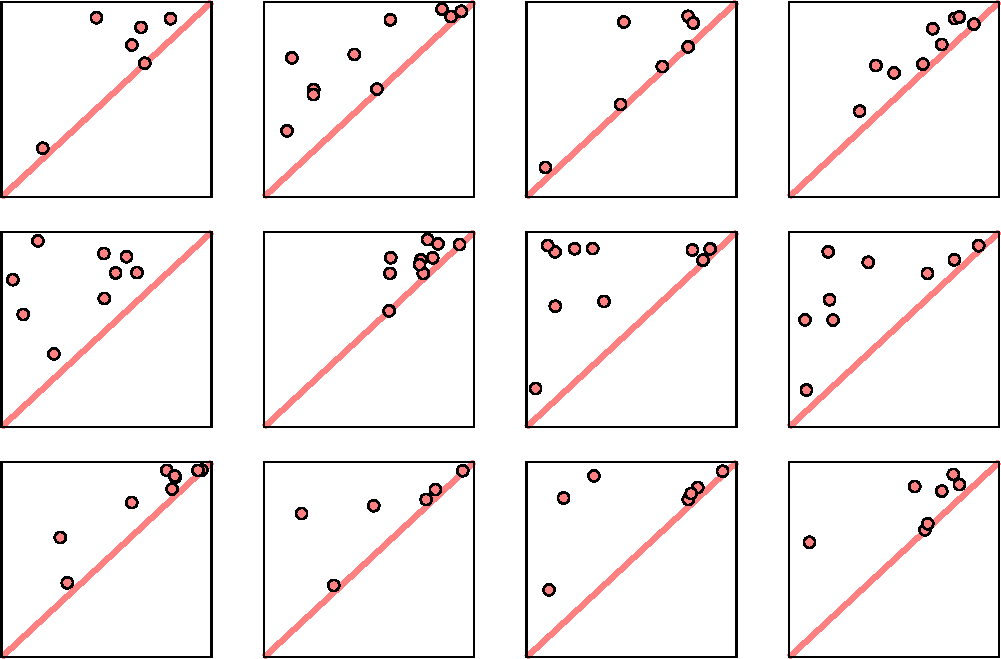
\includegraphics[width=.9\textwidth]{stat/sampling-dgms}}%
\end{block}
}

